\chapter{Background and related work}

To give some background to our method this chapter first gives a brief overview of machine learning and neural networks. Then, a selection of face detection, recognition, and reconstruction methods are presented. More emphasis is given to facial reconstruction methods, especially those that have been developed recently and use neural networks and synthetic data in one way or another.

% Finally, selected parts of computer graphics theory are presented.

\section{Machine learning and neural networks}

If we have a parametric function $f(\bm{x};\bm{\theta}) = \bm{y}$, how should the parameters $\bm{\theta}$ be adjusted so that, with input $\bm{x}$, the output of the function matches $\bm{y}$ as closely as possible? Machine learning, and especially its most common form, supervised machine learning, can be used to solve this problem. In supervised learning, the parameters $\bm{\theta}$ are iteratively adjusted until the output of the function cannot be further made more accurate. To make these kinds of small adjustments, a number of training pairs $(\bm{x}_i,\bm{y}_i)$ are needed in addition to some metric that tells how well the function is performing. \cite{Goodfellow2016,LeCun2015}

The function performance can be measured by a separate loss function that tells how far the output of the function is from the desired values. In the case of fitting a simple line function to a collection of points, the loss function could be visualized as the sum of the distances of the points from the line. If the points lie exactly on the line, the loss becomes zero, and further away the points are from the line, the bigger the loss becomes. Especially with more complex functions, the loss could be visualized as a multi-dimensional hilly landscape. Lower values of the loss function are valleys, and higher values are hills. The lower it is possible to travel in this loss landscape, the better the function under optimization performs. With complex functions, the loss landscape has numerous valleys and hills. Even if it seems that the loss is now small, because you are at the bottom of a valley, it is very much possible that there exists another valley somewhere else that is even deeper and thus better. \cite{Goodfellow2016,LeCun2015}

To adjust the parameters of the function, an algorithm called gradient descent is used. The gradient of the loss function can be visualized as an arrow that, at any point in the loss landscape, points towards the direction of the greatest ascent. To travel towards lower loss function values, that is, towards the bottoms of the valleys, a step into the opposite direction of the gradient should be taken. When repeated enough many times, a loss function minimum is reached. The problem with gradient descent is that, after reaching a bottom of a valley, the algorithm cannot continue. This means that the optimization could get stuck into a local minimum even though much better minima would be available further away. \cite{Goodfellow2016,LeCun2015}

If a very accurate gradient is calculated using all the available training data, it is very much possible for the gradient descent algorithm to get stuck at a local minimum. The accurate gradient calculation is also time-consuming and usually needs the whole dataset to be kept in memory. This is not feasible for very large datasets. The \ac{SGD} algorithm solves this problem by calculating a less accurate gradient from a smaller, randomly selected, part of the training dataset. This small selection of training samples is called a minibatch. The more random gradient is faster to calculate, and because it is noisy, it will help the gradient descent algorithm to escape from local minima. \cite{Goodfellow2016,LeCun2015}

Instead of using just one function as the target of the optimization, a composite of multiple functions, a network, can also be used. These networks are usually called neural networks because the functional parts are loosely inspired by neuroscience. A neural network has an input layer, any number of hidden layers, and an output layer. The adjacent layers can be fully connected to each other with distinct weights for each connection, and the values that flow through the network can be modified with activation functions. The hidden layers are called so because the training data does not give any desired output for them. Instead, when trained, the network is free to come up with its internal representations. The training of a neural network like this is enabled by the backpropagation algorithm. For it to work, one requirement is that the functions that compose the network are differentiable. If this is the case, the gradient calculated at the output layer can be backpropagated through the network, and all the parameters of the network can be adjusted accordingly. \cite{Goodfellow2016,LeCun2015}

The machine learning algorithms used today are largely the same as in the 1980s. The massive increase of computing power, storage space, and memory amounts in recent years has enabled the training of networks that were previously thought very hard to train. The modern general processing \acp{GPU} have been instrumental in making the training process faster, as their architecture suits the task very well. Some other smaller developments, e.g., using the \ac{RELU} activation function, have also played their part in making the training of deeper networks easier. Modern neural networks can have tens of millions of parameters, and the networks can be very deep with tens, if not hundreds, of layers. Deep learning, the name given to this new era of machine learning, reflects this fact. A good example of the deep learning advantage is the application of deep neural networks by \textcite{Krizhevsky2012} in the 2012 ImageNet competition. Their results were impressive, almost halving the error rate compared to the best competitors. \cite{Goodfellow2016,LeCun2015}

The functions that the network is composed of can also perform filtering using convolutions. These kinds of networks are called \acfp{CNN}. Convolutions can be though as small filters that are slid over the larger underlying signal and that produce a new, modified, signal. Convolutions are especially well suited for processing images. One of the first applications of \acp{CNN} was a method to recognize handwritten digits, developed by \textcite{Lecun1998}. Many convolutions, with differing filter values, can be applied to the same image. This allows the extraction of different features from the image. The hierarchical nature of the \acp{CNN} means that, at the first layers, the extracted features are edges, and then continuing deeper inside the network the features become parts, and parts become objects. The structure of \acp{CNN} has been directly inspired by the concepts in visual neuroscience. \cite{Goodfellow2016,LeCun2015}

An ordinary \ac{CNN} usually has fully connected layers at the end and will produce a one-dimensional vector as the final output \cite{Lecun1998}. In \acfp{FCNN}, the fully connected part at the end is replaced by a convolutional upsampling part \cite{Long2015}. This means that, for \acp{FCNN}, both the inputs and outputs can be images. \acp{FCNN} have been successfully used for dense image semantic segmentation. Semantic segmentation means understanding the image at the pixel level, i.e., giving each pixel of the input image a meaningful class \cite{Long2015,Ronneberger2015}. The training of \acp{FCNN} has been made easier with the introduction of the concept of skip connections. Skip connections connect the downsampling and upsampling parts of the \ac{FCNN} directly. Skip connections have been shown to help gradients propagate from the output towards the input side of the network, transfer high-frequency detail from the input side to output side, and help to avoid singularities in the loss landscape \cite{Ronneberger2015,Orhan2017,Goodfellow2016}.

Designing and training the neural networks, especially the deep ones, would be very time-consuming if the training code had to be reimplemented at low-level with every design iteration. To get fast enough training speeds, using \acp{GPU} is necessary. The training code has to be executable on \acp{GPU}, and efficient transfer of training data to the \acp{GPU} needs to be implemented. To help make the neural network design process, code generation for the \acp{GPU}, data transfer to the \acp{GPU}, and the training process easier, numerous software frameworks have been developed in recent years. Good examples of these software frameworks are \textcite{cntk}, \textcite{tensorflow}, and \textcite{pytorch}. With these frameworks, the neural network can be designed at high-level with the Python scripting language. Changes to the network topology can be made easily, and the framework will take care of converting the high-level network description into optimized low-level code that is ready to be run on \acp{GPU}. \cite{cntk,tensorflow,pytorch}

\section{Face detection and reconstruction}

The techniques for processing human faces in images are broadly classified into three categories by \textcite{Datta2015}: face detection, face recognition, and face reconstruction. Face detection tells us if there exists a human face in an image in the first place, and can give the approximate location and size of the face. Face recognition goes a step further as it can identify the actual person in the image. Face reconstruction does not necessarily have anything to do with identification but rather finding out the underlying facial geometry, i.e., the facial shape, of the human pictured.

\begin{figure}
    \centering
    \subfloat[\cite{Sakai1972}]{\label{fig:face_detection_1a}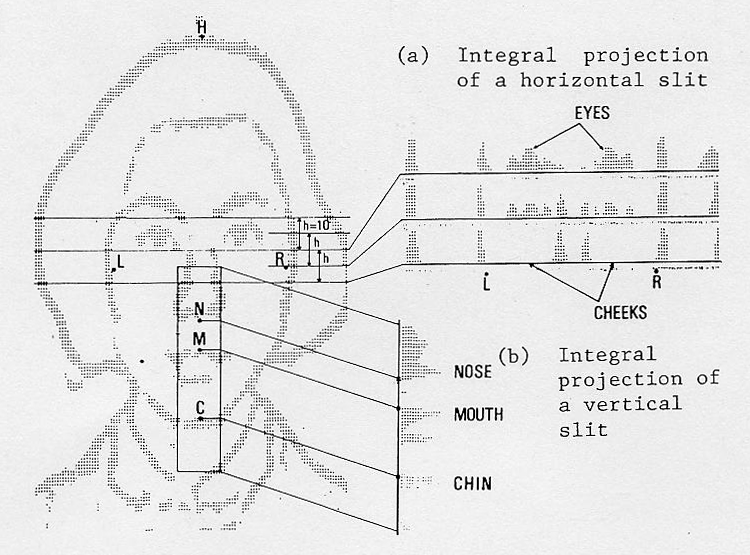
\includegraphics[height=.3\textwidth]{takeo}}\qquad\qquad
    \subfloat[]{\label{fig:face_detection_1b}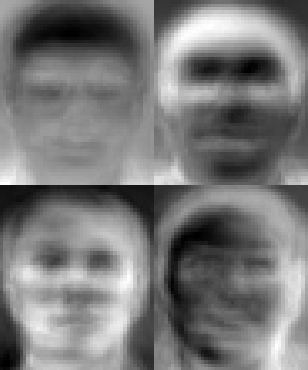
\includegraphics[height=.3\textwidth]{eigenfaces}}
    \caption[Face detection 1]{One of the first face detection systems was developed in the early 1970s by \textcite{Sakai1972}. Their algorithm was based on analyzing slices of a binary image of the head as shown in \protect\subref{fig:face_detection_1a}. Face recognition based on eigenfaces, as proposed by \textcite{Turk1991}, was one of the first commercially viable methods for face recognition. Visualizations of eigenfaces are shown in \protect\subref{fig:face_detection_1b} (Copyright of AT\&T Laboratories Cambridge).}
    \label{fig:face_detection_1}
\end{figure}

One of the first automated face detection systems was developed in the early 1970s by \textcite{Sakai1972}. The input was a 5-bit grayscale image with a resolution of 140x208. The image was processed with an edge detecting filter and then thresholded to obtain a binary image containing contours of the face. See figure \ref{fig:face_detection_1a} for an example. The binary image was then scanned slice-by-slice from top to bottom. Each slice was analyzed while an elaborate state machine kept track whether the image contained a human or not. The face had to be centered in the image and could have only a small amount of tilt in any direction. This method did not work at all if the person in the image had glasses or a beard.

The method of using eigenfaces for recognizing humans from pictures was introduced by \textcite{Turk1991} in 1991. It was one of the first accurate and fast enough methods to be used commercially. The method captured the relevant variation in a collection of facial images, that is, the principal components of the distribution, into eigenvectors. The eigenvectors can be visualized as ghostly faces, eigenfaces, as is shown in figure \ref{fig:face_detection_1b}. Any picture of a human face could then be deconstructed into a linear combination of eigenvectors, and inversely, reconstructed with the same linear combination of the same eigenvectors. The face recognition could be done by comparing the weights of the linear combinations as the weights would be similar between two images of the same person.

\begin{figure}
    \centering
    \subfloat[\cite{Viola2001}]{\label{fig:face_detection_2a}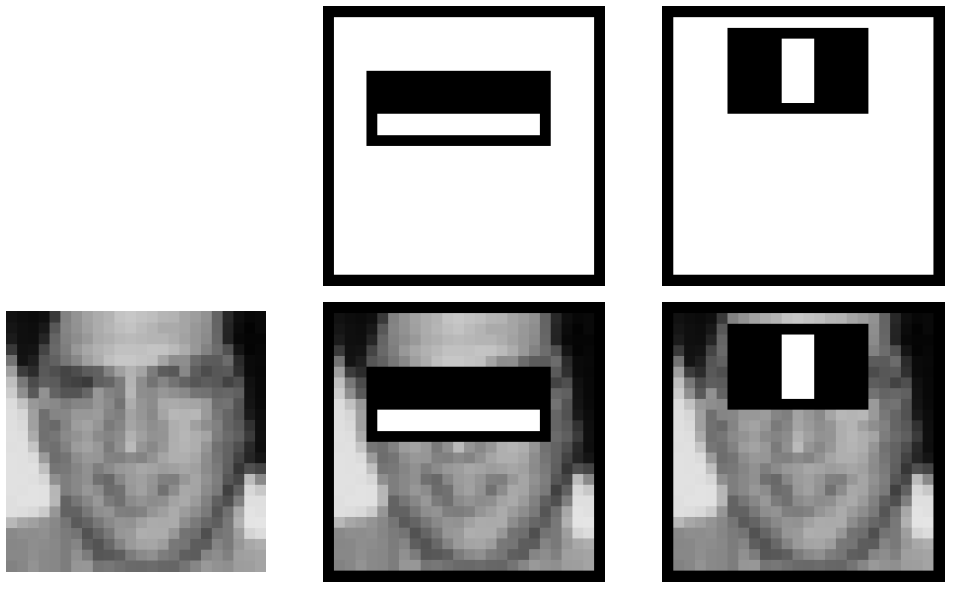
\includegraphics[height=.28\textwidth]{viola}}\hfill
    \subfloat[ \cite{Osadchy2007}]{\label{fig:face_detection_2b}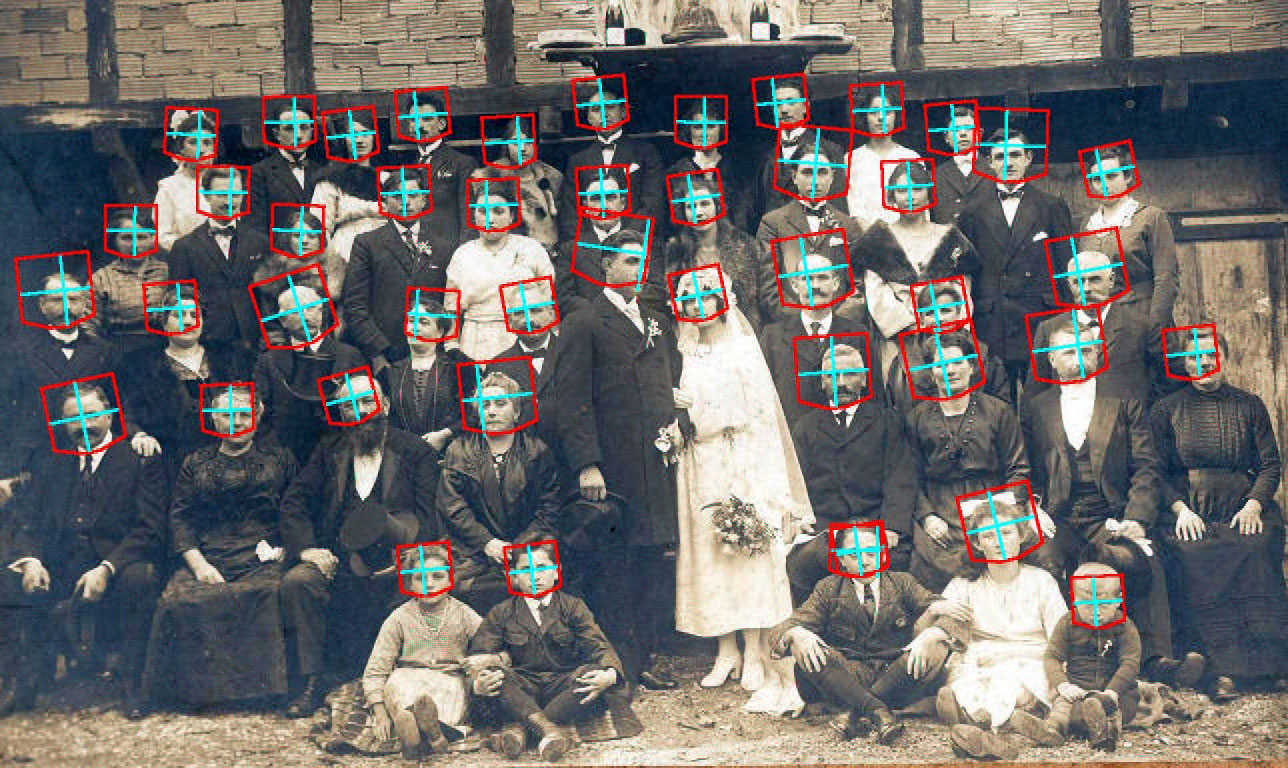
\includegraphics[height=.28\textwidth]{osadchy}}
    \caption[Face detection 2]{Face detection speed was greatly increased by a method introduced by \textcite{Viola2001}. The method was based on fast evaluation of rectangular filters and machine learning. Some filters are visualized in \protect\subref{fig:face_detection_2a}. Convolutional neural networks were used by \textcite{Osadchy2007} for fast face detection and pose estimation. \protect\subref{fig:face_detection_2b} shows how the algorithm performed on a somewhat difficult image.}
    \label{fig:face_detection_2}
\end{figure}

The speed of detecting faces and generating the bounding boxes around them was dramatically improved by \textcite{Viola2001} in 2001. Their proposed method was based on the idea of the integral image, rectangular feature filters, and machine learning. The integral image, or summed area tables, was an intermediate representation of the image that allowed rapid summation of pixels in arbitrary rectangular areas. The rectangular feature filters are illustrated in figure \ref{fig:face_detection_2a}. The filter calculated the sum of the pixels in the white area which was then subtracted from the sum of the black area. The filter could thus find intensity variations between arbitrary rectangular areas rapidly. Hundreds of thousands of possible combinations of these filters existed for a 24x24 pixel detection window, and machine learning was used to select few thousand of the most relevant filters for human face detection. Applying the resulting combination of filters to images was fast, and faces could be detected and tracked near real-time with contemporary hardware.

In 2007, \textcite{Osadchy2007} published a novel method for simultaneously detecting faces and estimating their poses in real-time using convolutional neural networks. Figure \ref{fig:face_detection_2b} shows how the network was able to detect multiple faces in one image including their yaw from left to right and in-plane rotation. Their network topology was similar to the one used by \textcite{Lecun1998} in 1998 to recognize hand-written digits. The training data consisted of real human faces which were manually annotated with the pose data. The method could do face detection and pose estimation at the same time quicker and more accurately than previous methods that did the tasks separately.

\begin{figure}
    \centering
    \subfloat[\cite{Blanz1999}]{\label{fig:face_reconstruction_1a}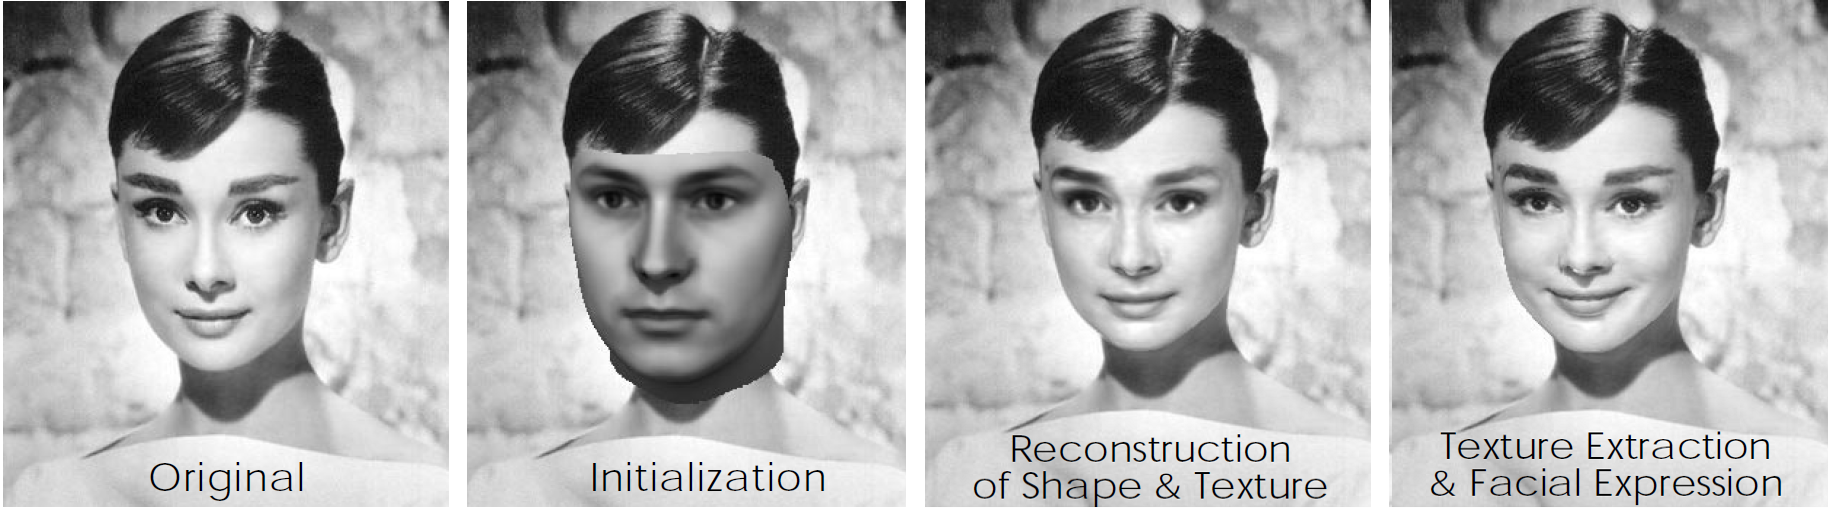
\includegraphics[height=.2\textwidth]{blanz}}
    
    \subfloat[\cite{Richardson2016a}]{\label{fig:face_reconstruction_1b}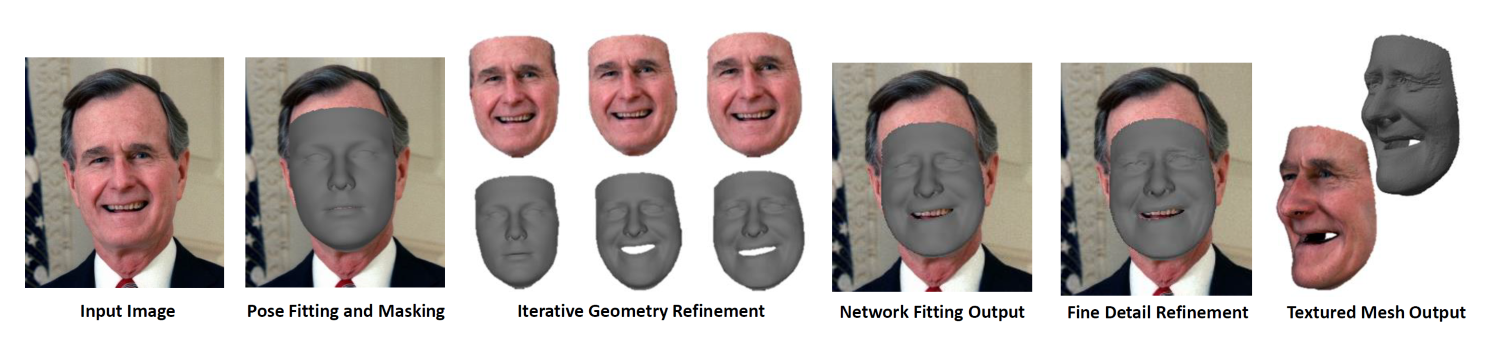
\includegraphics[width=\textwidth]{richardson1}}
    \caption[Face reconstruction 1]{Facial geometry and texture reconstruction using a 3D morphable model was proposed by \textcite{Blanz1999}. The steps of their algorithm are shown in \protect\subref{fig:face_reconstruction_1a}. \textcite{Richardson2016a} used a \ac{CNN} and an iteration process to fit the morphable model to the input image. The steps are shown in \protect\subref{fig:face_reconstruction_1b}.}
    \label{fig:face_reconstruction_1}
\end{figure}

In 1999, \textcite{Blanz1999} introduced a new technique to reconstruct human facial geometry from a single image using a 3D morphable face model. They started by scanning hundreds of real human faces with a 3D laser scanner. The scan produced accurate vertex positions and colors. The generated 3D face models were processed so that they all came into full correspondence with each other. Using \ac{PCA} decomposition, an average face model and a set of basis face vectors were created. \ac{PCA} was also done for the vertex color data. This allowed a parametric creation of 3D face models and their textures. The process of reconstructing the facial geometry from a single image started with a coarse manual alignment of the average face model over the image. An analysis-by-synthesis loop was then repeated where the face model was rendered over the image, and the factors of the principal components were adjusted until an optimization minimum was reached. Finally, additional detailed facial texture information was extracted from the image as the color \ac{PCA} components did not contain enough high-resolution data. Steps of this process are shown in figure \ref{fig:face_reconstruction_1a}.

More recently, in 2016, \textcite{Richardson2016a} proposed a method to extract 3D morphable model parameters from real-world images using a \ac{CNN}. The steps of their algorithm are visualized in figure \ref{fig:face_reconstruction_1b}. They started by aligning the average morphable face model over the image using another posing algorithm. The face was segmented out of the background and fed to the \ac{CNN} along with a rendered version of the current morphable face model. The \ac{CNN} was trained to output a correction term to the morphable model parameters to make the rendered face model match the segmented real face image better. The face model rendering and parameter correction calculation were repeated iteratively multiple times to increase the quality of the reconstruction. The \ac{CNN} was completely trained on synthetic data generated using the 3D morphable face model. Because fine facial details could not be extracted using this method, they were later captured with a separate shape-from-shading algorithm.

\textcite{Richardson2016} improved their previous method of \cite{Richardson2016a}. The problem with their previous method was that it needed separate initialization of the average face model over the input image and that the method could not extract fine details without an external algorithm. The improved algorithm could do both in one go using two connected networks, a \ac{CNN} and an \ac{FCNN}. The \ac{CNN} was applied iteratively to the input image and a coarse geometry using a 3D morphable model was recovered. A depth map was generated from this model, and the map was fed to the \ac{FCNN} along with the input image. The \ac{FCNN} was trained to do fine detail reconstruction, i.e., shape-from-shading, within the depth map in one shot without iteration. The \ac{CNN} was trained in a supervised manner with synthetic data rendered using the 3D morphable model, and the \ac{FCNN} was trained in an unsupervised manner using real-world images.

\textcite{Kim2017} introduced a method that could estimate a wide variety of 3D morphable model parameters from a real-world image in a single shot using a \ac{CNN}. The estimated parameters included facial pose, facial shape, facial expression, skin reflectance, and scene illumination. No iteration was needed to refine the results. Before feeding the real-world images to the network, their variety was reduced by segmenting the faces out of the backgrounds using facial landmark detection. The network was trained exclusively on synthetic training data derived from the 3D morphable model. To get the parameter distributions of the synthetic training data to better model the real-world distributions, a novel breeding method was introduced that used real-world facial images to update the training set. A network trained with the breeding outperformed a network trained only on synthetic data.

\textcite{Tewari2017} were able to train an autoencoder \ac{CNN} completely unsupervised using only real-world images. No separately generated synthetic data was used. The \ac{CNN} was able to extract 3D morphable model parameters including facial pose, facial shape, facial expression, skin reflectance, and scene illumination in a single iteration. The method relied on a novel analytical and differentiable decoder layer that used the morphable model parameters to reconstruct the input image. It was possible to train the network in an unsupervised manner because the loss could be backpropagated through the decoder layer. With a method like this, the real-world distribution of the morphable model parameters could be captured the best, and the network could generalize well to real-world images.

\begin{figure}
    \centering
    \subfloat[\cite{Sela2017}]{\label{fig:face_reconstruction_2a}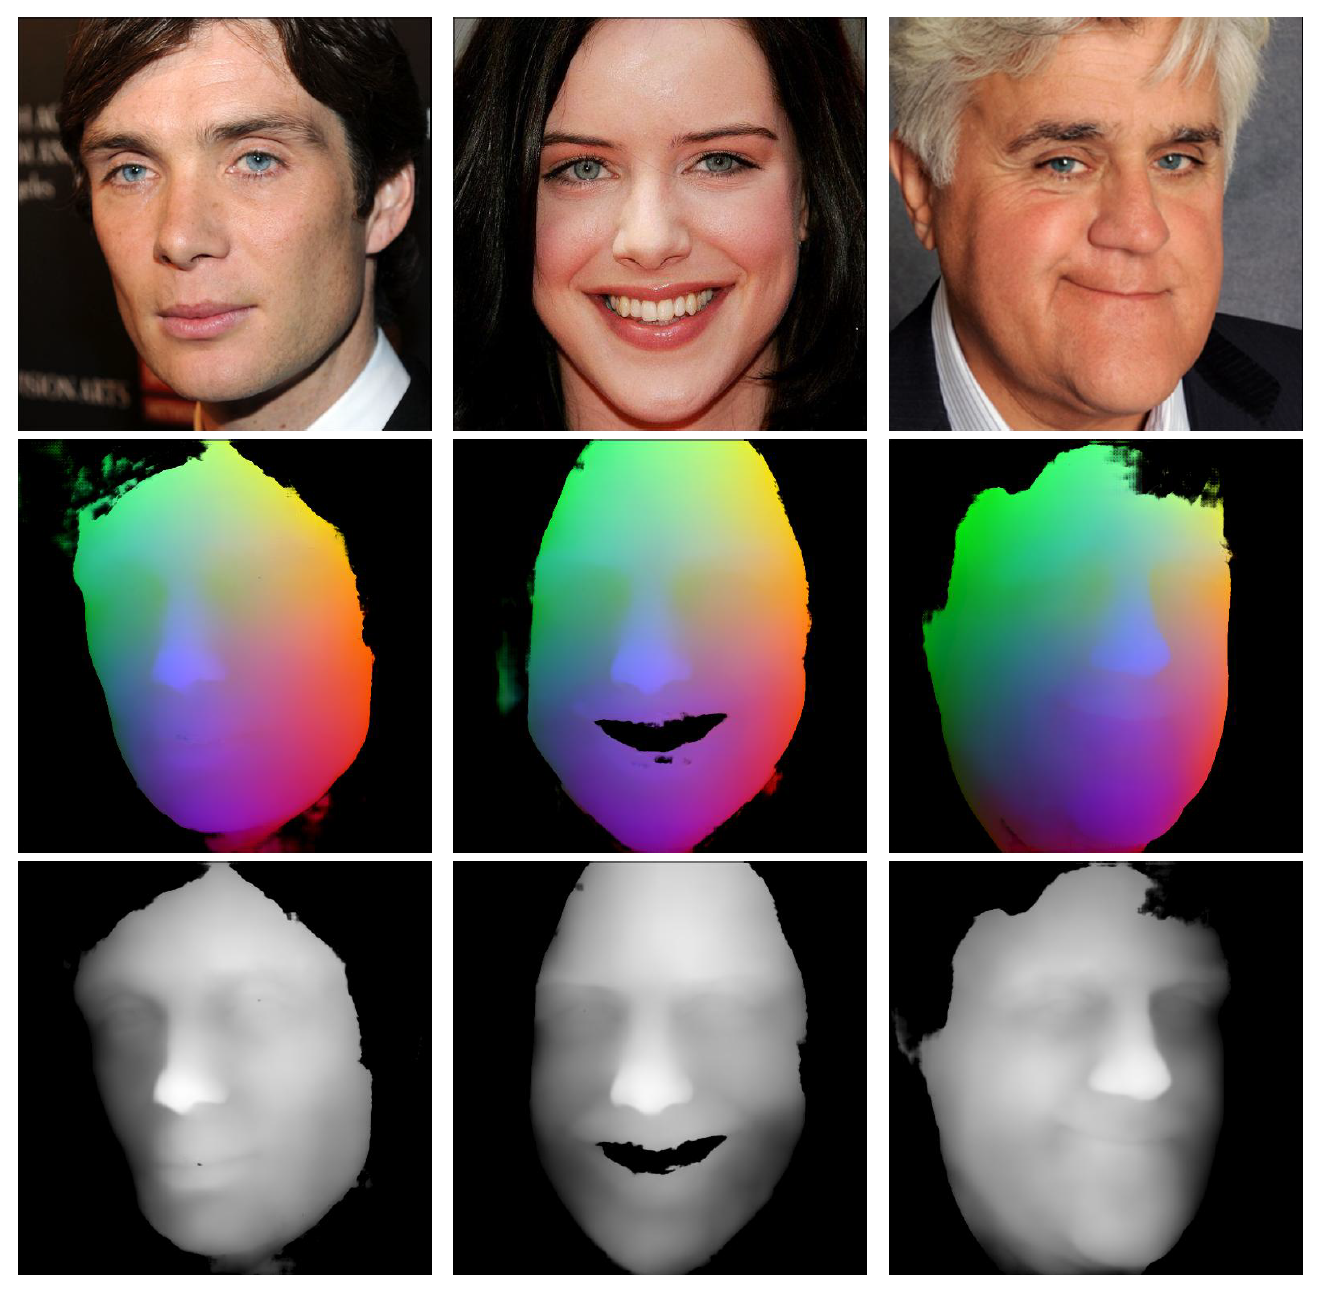
\includegraphics[height=.3\textwidth]{sela1}}\qquad\qquad
    \subfloat[\cite{Guler2016}]{\label{fig:face_reconstruction_2b}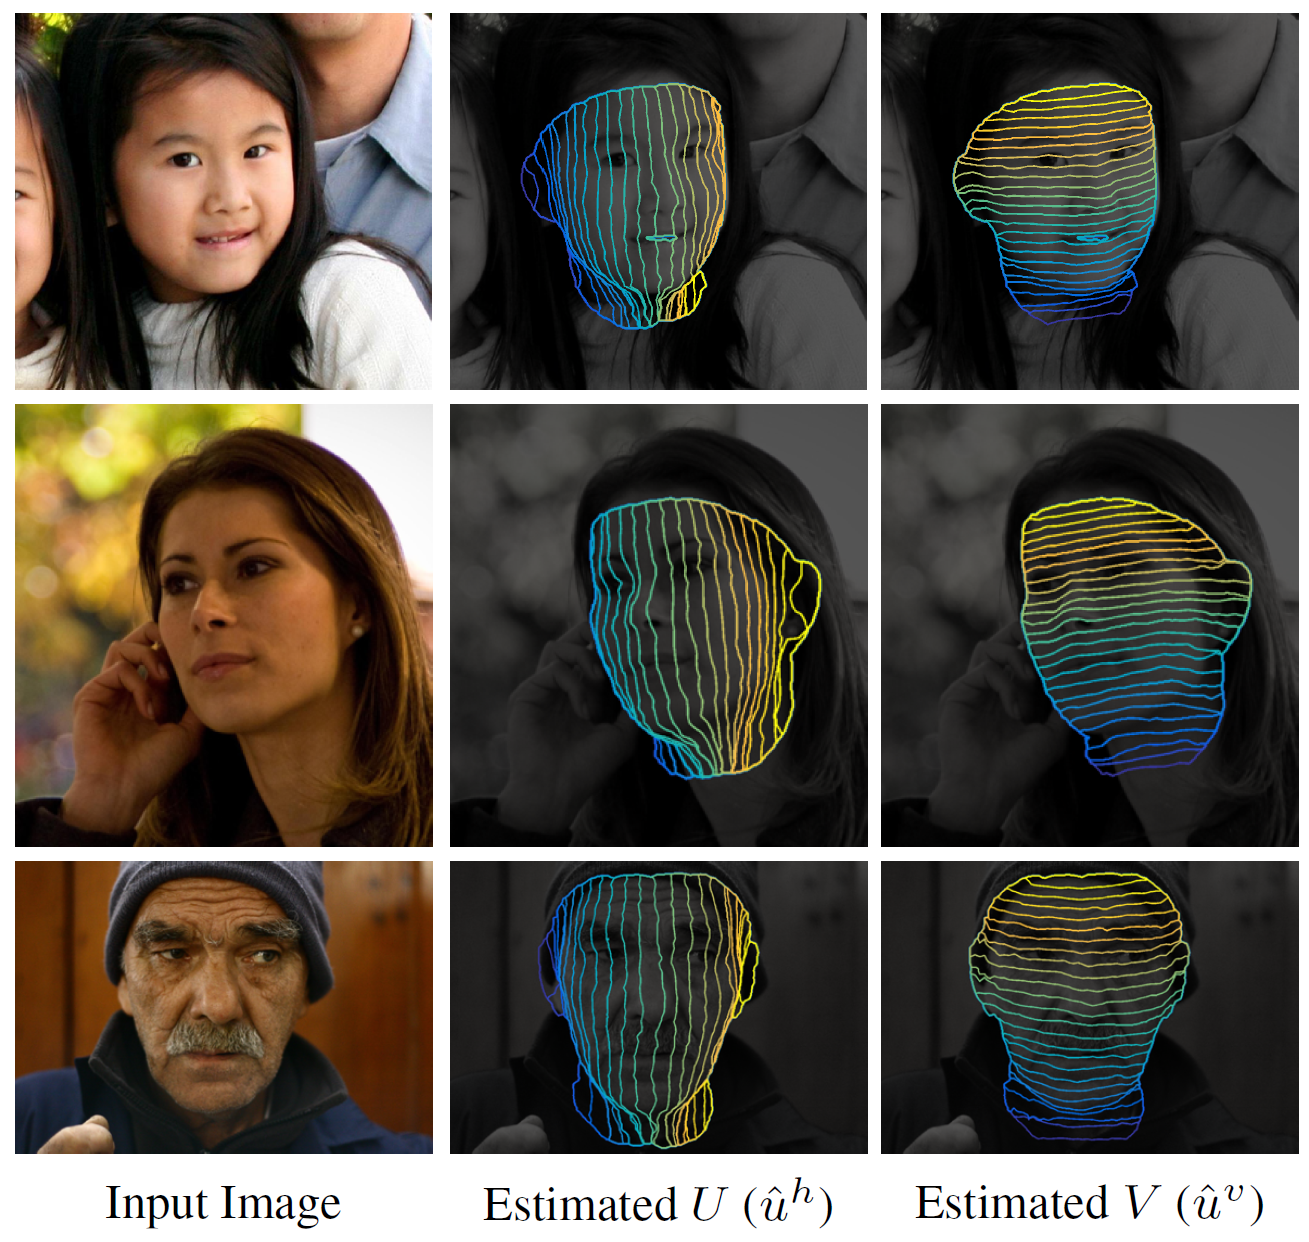
\includegraphics[height=.3\textwidth]{guler1}}
    
    \subfloat[\cite{Yu2017}]{\label{fig:face_reconstruction_2c}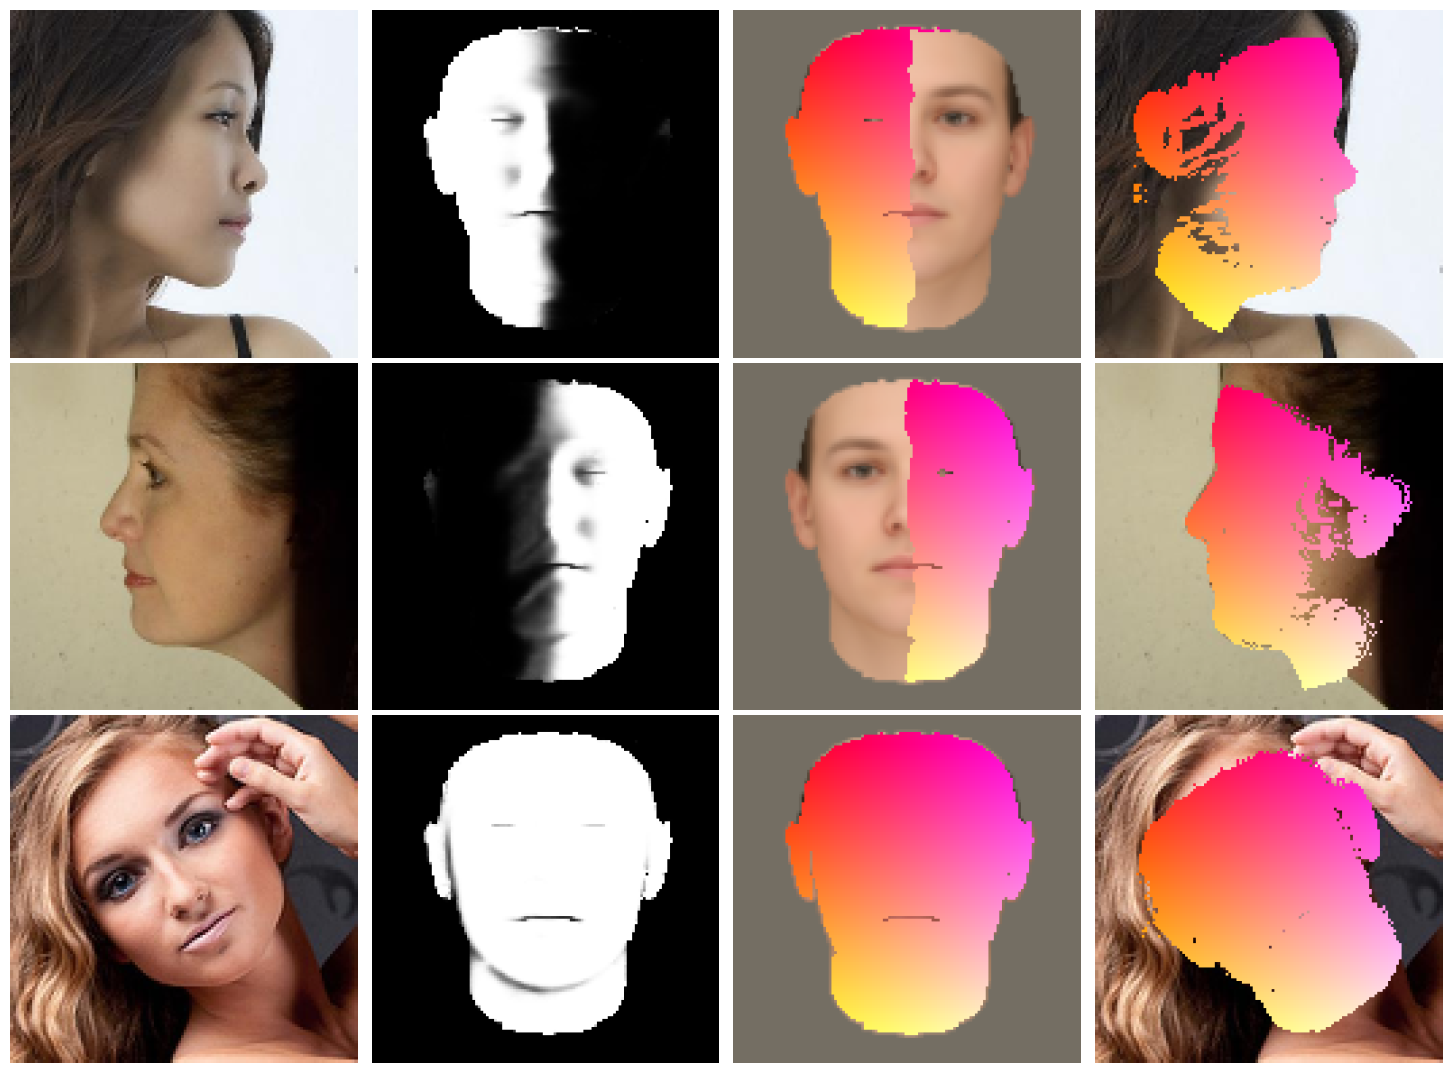
\includegraphics[height=.3\textwidth]{yu1}}
    \caption[Face reconstruction 2]{The method of \textcite{Sela2017} generated dense correspondence and depth map images. Their results are shown in \protect\subref{fig:face_reconstruction_2a}. \textcite{Guler2016} generated dense correspondences using quantized regression which resulted in outputs shown in \protect\subref{fig:face_reconstruction_2b}. \textcite{Yu2017} proposed a method that could estimate dense 2D pixel flow between the input image and a front-facing template mesh. Visualization of their method is shown in \protect\subref{fig:face_reconstruction_2c}.}
    \label{fig:face_reconstruction_2}
\end{figure}

After the work on this thesis had started, multiple papers were published that had similar ideas regarding \acp{CNN} and dense geometry generation. \textcite{Sela2017} proposed an \ac{FCNN} that could map a real-world human face image to a dense correspondence image and a dense depth map image. Examples of these images are shown in figure \ref{fig:face_reconstruction_2a}. In contrast to most of the previously mentioned methods, this method did not use a 3D morphable model in the reconstruction process. The correspondence and depth map images were then used with a separate algorithm to extract the 3D mesh of the face. The network was trained with synthetic data with a wide range of facial shapes, facial poses, facial materials, lighting conditions, and background textures. A surprising result was that even though the synthetic data was created with a limited generative model, the network could generalize beyond the limited scope of the training material.

\textcite{Guler2016} trained an \ac{FCNN} to estimate dense correspondences between image pixels and a 3D template mesh projected onto a 2D deformation-free space, or in other words, a UV space. Their approach was very similar to ours, but instead of plain regression, they used quantized regression. The mappings generated by this method are illustrated in figure \ref{fig:face_reconstruction_2b}. The training dataset was generated from real-world images that had existing facial landmark annotations. The dataset generation was done by first fitting the 3D template mesh over the image using the landmarks and then rasterizing the mesh using colors representing locations in the deformation-free space.

\textcite{Yu2017} used an \ac{FCNN} to generate dense facial correspondences between the input image and a 3D morphable face model. Two images were generated from the input image: a 2D flow image and a matchability mask image. The 2D flow image estimated the flow between the input image pixels and a synthetic rendering of an average frontal face. The matchability image indicated which correspondences were valid inside the average face. These images are visualized in figure \ref{fig:face_reconstruction_2c}. In the beginning, the network was trained with synthetic data generated from a 3D morphable model. Later, the network was refined using annotated real-world images. Simple rectangular occlusions were also added to the training data which made the model more robust against obstructions over the faces.

\begin{figure}
    \centering
    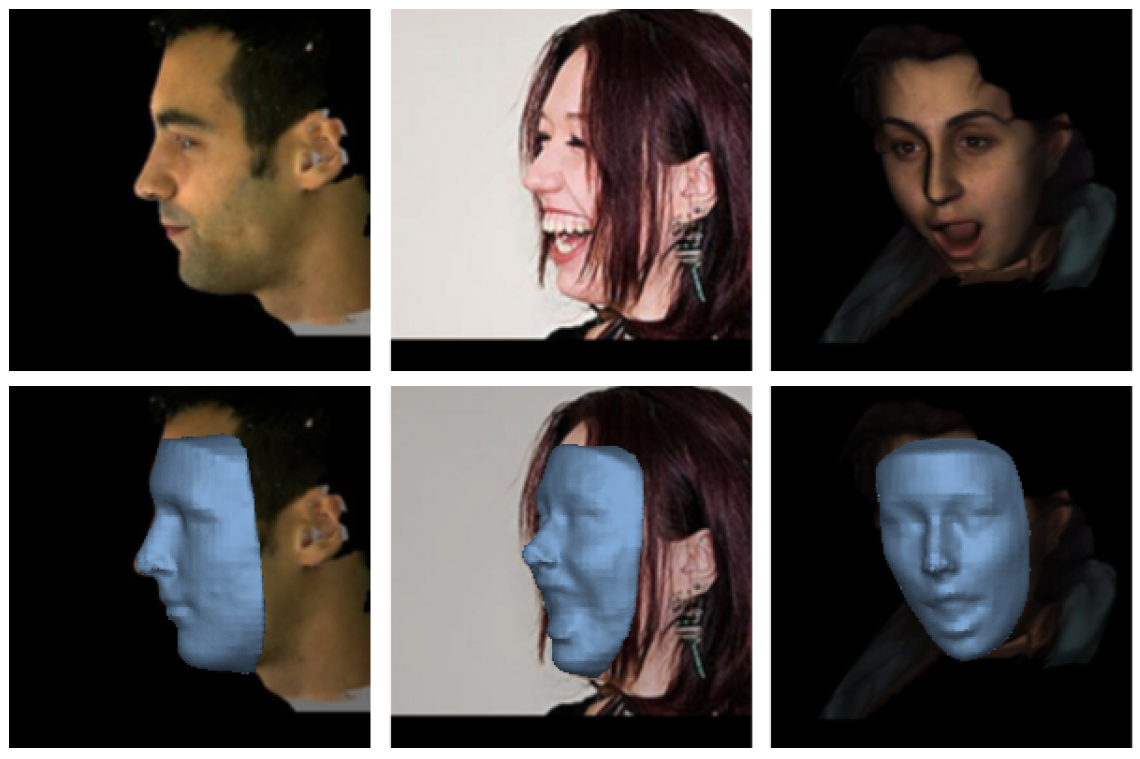
\includegraphics[height=.4\textwidth]{jackson1}
    \caption[Face reconstruction 3]{Results of the method proposed by \textcite{Jackson2017}. They used \acp{FCNN} to regress from the input image into a 3D volume directly.}
    \label{fig:face_reconstruction_3}
\end{figure}

In late 2017, \textcite{Jackson2017} published a novel method that used \acp{FCNN} for direct 2D-to-3D facial geometry reconstruction. No intermediate fitting steps were used. The training dataset consisted of real-world images and corresponding 3D binary volumes that modeled the faces in the input images. Inside the volume, if a voxel was inside the face, it was given a value of 1, and 0 otherwise. The 3D binary volumes were created using a 3D morphable model that was already fitted to the input images. The actual 3D facial geometry was recovered by generating the iso-surface of the regressed binary volume. Results of this method are shown in figure \ref{fig:face_reconstruction_3}.

\iffalse

\section{Computer graphics and rendering}

Computer graphics theory is a vast subject area. The relevant parts of it, for this thesis, are 3D mesh representation, texture mapping, surface reflectance models (\acsp{BRDF}), the light transport equation, path tracing, and antialiasing.

\begin{gather}
L_o(p, \omega_o) = L_e(p, \omega_o) + \int_\Omega f(p, \omega_o, \omega_i) L_i(p, \omega_i) |cos\theta_i| d\omega_i
\end{gather}

\begin{Verbatim}
- how 3D meshes are composed of triangles
- triangles have vertices that have 3D world coordinates and 2D UV coordinates
- UV coordinates are used for texture mapping
- rendering can be performed by shooting rays from the camera
- realistic images can be generated by solving the lighting equation
- lighting equation can be solved using path tracing
- light bouncing determined by surface reflectance models (BRDFs)
- reflectance models (BRDFs)
- smoothing edges using antialiasing
\end{Verbatim}

\begin{figure}[h]
    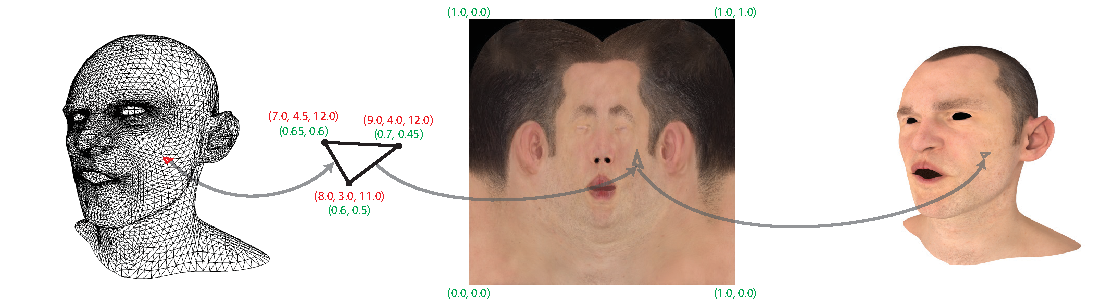
\includegraphics[width=\textwidth]{tex-mapping}
    \caption[Texture mapping]{An illustration of the texture mapping process. A 3D mesh consists of triangles. Each vertex of a triangle usually has at least a 3D world coordinate (red) and a 2D UV coordinate (green). UV coordinates map the triangle onto the 2D UV space of the texture. The color from the texture can be applied to the triangle when rendering.}
    \label{fig:tex_mapping_1}
\end{figure}

\fi
